% ---------------------------------------------------------------------------
% Chapter -- Kinematic Model
%
% Being rewritten paragraph by paragraph in plain, impersonal English.
% Formulas were re-derived symbolically (sympy), agree with the MATLAB code
% (fields_exact) and with Zuyev & Grushkovskaya, arXiv:2403.03341, Sec. II.
% ---------------------------------------------------------------------------

\chapter{Kinematic Model}
\label{ch:model}

This chapter derives the equations of motion of a differential-drive robot
that pulls two trailers. Each trailer is hitched at a point that does not lie
on the axle of the vehicle in front of it. The result is a driftless
control-affine system with five states and two inputs. Then it is shown that the
system is locally controllable, and its degree of nonholonomy is computed.
Finally, the reduced system with a single trailer is stated.

The model is taken from~\cite{zuyev2024}, where the result is stated without
intermediate steps. The derivation below fills in those steps. The notation is
introduced in Section~\ref{sec:geometry}.

% ===========================================================================
\section{Geometry and notation}
\label{sec:geometry}

The system has three parts: the robot and two trailers. Each part has one pair
of wheels on a common axle. Let $C_0$, $C_1$ and $C_2$ be the midpoints of the
three axles. Let $\varphi$, $\theta_1$ and $\theta_2$ be the angles that the
robot, the first trailer and the second trailer point to. They are measured
counter-clockwise from the $x$-axis of a fixed coordinate system
(\cref{fig:geometry}).

The parts are connected by two hitches, $H_1$ and $H_2$. Each hitch is a hinge
that turns around a vertical axis, so a trailer can swing left and right. The
geometry is described by four lengths. Each one is measured along the part it
belongs to:
\begin{itemize}
  \item $\dzero$ -- from $C_0$ to the first hitch $H_1$,
  \item $\lone$ -- from $H_1$ to the axle midpoint $C_1$,
  \item $\done$ -- from $C_1$ to the second hitch $H_2$,
  \item $\ltwo$ -- from $H_2$ to the axle midpoint $C_2$.
\end{itemize}

\begin{figure}[t]
  \centering
  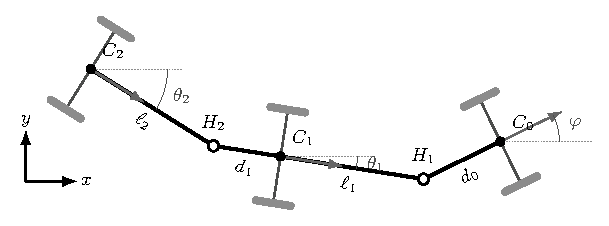
\includegraphics[width=0.85\textwidth]{geometry.pdf}
  \caption{Geometry of the car with two off-hooked trailers. $C_0,C_1,C_2$
  are the axle midpoints, $H_1,H_2$ the hitches, $\varphi,\theta_1,\theta_2$
  the headings measured from the $x$-axis. Proportions are exaggerated for
  legibility.}
  \label{fig:geometry}
\end{figure}

\begin{definition}[Off-hooked trailer]
\label{def:offhooked}
A trailer is \emph{off-hooked} if its hitch is not on the axle of the vehicle in
front of it. In \cref{fig:geometry} this means $\dzero>0$ for the first trailer
and $\done>0$ for the second.
\end{definition}

Off-hooked trailers are harder to control than trailers hitched on the axle.
If $\dzero=\done=0$, the equations can be changed into a simple standard form
called the chained form \cite{sordalen1993}, and there are well-known methods
for controlling it. With off-hooked trailers this is not possible. This is
discussed in Chapter~\ref{ch:background}. What it means for the controller is
explained at the end of \cref{sec:controllability}.

The configuration is collected in the state vector
\begin{equation}
  x=(x_1,x_2,x_3,x_4,x_5)^\top
   =(x_{C_0},\,y_{C_0},\,\varphi,\,\theta_1,\,\theta_2)^\top\in\R^5,
  \label{eq:state}
\end{equation}
where $(x_{C_0},y_{C_0})$ are the coordinates of $C_0$. For an angle $\alpha$, let
$e(\alpha)=(\cos\alpha,\sin\alpha)^\top$ be the unit vector pointing in that
direction. Let $e^\perp(\alpha)=(-\sin\alpha,\cos\alpha)^\top$ be the unit
vector at a right angle to it. Note that $\dot e(\alpha)=\dot\alpha\,e^\perp(\alpha)$.

% ===========================================================================
\section{Rolling-without-slipping constraints}
\label{sec:rolling}

It is assumed that the wheels roll without slipping. This means that a part can
move forward or backward and can turn, but it cannot slide sideways. Take one
part. Let $\alpha$ be the angle it points to, and let $C=(x_C,y_C)$ be the
midpoint of its axle. The sideways direction is $e^\perp(\alpha)$. The sideways
component of the velocity of $C$ is $\dot C\cdot e^\perp(\alpha)$, and it
must be zero:
\begin{equation}
  \dot x_C\sin\alpha-\dot y_C\cos\alpha=0 .
  \label{eq:oneaxle}
\end{equation}

Applied to all three parts, this gives
\begin{align}
  \dot x_{C_0}\sin\varphi-\dot y_{C_0}\cos\varphi&=0,\label{eq:rolling0}\\
  \dot x_{C_1}\sin\theta_1-\dot y_{C_1}\cos\theta_1&=0,\label{eq:rolling1}\\
  \dot x_{C_2}\sin\theta_2-\dot y_{C_2}\cos\theta_2&=0.\label{eq:rolling2}
\end{align}

The state has five numbers, and these are three independent rules that the
motion must follow. So at each moment only two directions of motion are free.
The other three can only be reached by combining the two inputs in sequences of
movements (\cref{sec:controllability}).

% ===========================================================================
\section{Trailer axle positions}
\label{sec:positions}

The first hitch $H_1$ is behind $C_0$, at the distance $\dzero$ in the direction
of the robot: $H_1=C_0-\dzero\,e(\varphi)$. The axle midpoint $C_1$ is a further
$\lone$ behind $H_1$, in the direction of the first trailer. The second hitch
$H_2$ is $\done$ behind $C_1$, in the same direction, and $C_2$ is $\ltwo$ behind
$H_2$, in the direction of the second trailer. This gives
\begin{align}
  C_1&=C_0-\dzero\,e(\varphi)-\lone\,e(\theta_1),\label{eq:C1}\\
  C_2&=C_0-\dzero\,e(\varphi)-(\lone+\done)\,e(\theta_1)-\ltwo\,e(\theta_2).
  \label{eq:C2}
\end{align}
The minus signs mean ``behind'', because $e(\alpha)$ points forward. The lengths
$\lone$ and $\done$ both lie along the first trailer, so in the second equation
they are added together.

% ===========================================================================
\section{Driftless control-affine system}
\label{sec:affine}

The equations of motion follow from the rolling rules. The robot has two
inputs. The first, $u_1$, is how fast it drives forward. The second, $u_2$, is
how fast it turns, in radians per second. The first rolling rule says that the
velocity of $C_0$ points in the direction the robot faces, so
$\dot C_0=u_1\,e(\varphi)$. In coordinates this is
\begin{equation}
  \dot x_1=u_1\cos x_3,\qquad \dot x_2=u_1\sin x_3,\qquad \dot x_3=u_2 .
  \label{eq:robot}
\end{equation}
The first two equations say how the position changes, and the third says that
the angle of the robot changes at the speed $u_2$.

\paragraph{First trailer.}
The first trailer must also not slide sideways. To use this rule, the
velocity of $C_1$ is needed. It is obtained by taking the derivative
of~\eqref{eq:C1}, using $\dot e(\alpha)=\dot\alpha\,e^\perp(\alpha)$:
\begin{equation}
  \dot C_1=\dot C_0-\dzero\,\dot\varphi\,e^\perp(\varphi)
          -\lone\,\dot\theta_1\,e^\perp(\theta_1).
\end{equation}
The rolling rule~\eqref{eq:rolling1} for the first trailer says
$\dot C_1\cdot e^\perp(\theta_1)=0$. The relations $\dot C_0=u_1\,e(\varphi)$ and
$\dot\varphi=u_2$ are put in. Two dot products are also needed:
\begin{equation}
  e(\varphi)\cdot e^\perp(\theta_1)=\sin(\varphi-\theta_1),\qquad
  e^\perp(\varphi)\cdot e^\perp(\theta_1)=\cos(\varphi-\theta_1).
\end{equation}
Then the rule becomes
\begin{equation}
  u_1\sin(\varphi-\theta_1)-\dzero u_2\cos(\varphi-\theta_1)-\lone\dot\theta_1=0.
\end{equation}
Solving for $\dot\theta_1$ gives
\begin{equation}
  \dot x_4=\frac{u_1\sin(x_3-x_4)-\dzero\,u_2\cos(x_3-x_4)}{\lone}.
  \label{eq:x4dot}
\end{equation}
The second term comes from the off-hooked hitch. If $\dzero=0$, the input $u_2$
does not change the trailer angle. If $\dzero>0$, turning the robot on the spot
already pulls the trailer around.

\paragraph{Second trailer.}
The second trailer works in the same way. The derivative
of~\eqref{eq:C2} is
\begin{equation}
  \dot C_2=\dot C_0-\dzero\,\dot\varphi\,e^\perp(\varphi)
          -(\lone+\done)\,\dot\theta_1\,e^\perp(\theta_1)
          -\ltwo\,\dot\theta_2\,e^\perp(\theta_2).
\end{equation}
The rolling rule~\eqref{eq:rolling2} for the second trailer says
$\dot C_2\cdot e^\perp(\theta_2)=0$. The same kind of dot products is needed
as before. The new one is
$e^\perp(\theta_1)\cdot e^\perp(\theta_2)=\cos(\theta_1-\theta_2)$. Then the rule
becomes
\begin{equation}
  u_1\sin(\varphi-\theta_2)-\dzero u_2\cos(\varphi-\theta_2)
  -(\lone+\done)\,\dot\theta_1\cos(\theta_1-\theta_2)-\ltwo\,\dot\theta_2=0 .
\end{equation}
The term with $\dot\theta_1$ is new. It appears because the first trailer pulls
the second one, so when the first trailer turns, it moves the second one too. Solving
for $\dot\theta_2$ and putting in~\eqref{eq:x4dot} gives $\dot x_5$ as a
combination of $u_1$ and $u_2$, with the coefficients $f_{15}$ and $f_{25}$
below.

\paragraph{Result.}
The five equations of motion all have the form ``a function of $x$ times $u_1$,
plus another function of $x$ times $u_2$''. The first functions form the column
$f_1$, and the second functions form the column $f_2$. So the whole system is
\begin{equation}
  \dot x=u_1f_1(x)+u_2f_2(x),\qquad x\in\R^5,\ u\in\R^2,
  \label{eq:system}
\end{equation}
with
\begin{equation}
  f_1(x)=\begin{pmatrix}\cos x_3\\ \sin x_3\\ 0\\
        \dfrac{\sin(x_3-x_4)}{\lone}\\ f_{15}(x)\end{pmatrix},\qquad
  f_2(x)=\begin{pmatrix}0\\ 0\\ 1\\
        -\dfrac{\dzero\cos(x_3-x_4)}{\lone}\\ f_{25}(x)\end{pmatrix},
  \label{eq:fields}
\end{equation}
\begin{align}
  f_{15}(x)&=\frac{\sin(x_3-x_5)}{\ltwo}
     -\frac{(\done+\lone)\sin(x_3-x_4)\cos(x_4-x_5)}{\lone\ltwo},\\
  f_{25}(x)&=\frac{\dzero(\done+\lone)\cos(x_3-x_4)\cos(x_4-x_5)}{\lone\ltwo}
     -\frac{\dzero\cos(x_3-x_5)}{\ltwo}.
\end{align}
A system of this form is called \emph{driftless} and \emph{control-affine}.
Driftless means that nothing moves when $u_1=u_2=0$. Control-affine means that
the inputs only multiply functions of the state, and the results are added.

This system has two important features.

First, $\dot x_3=u_2$ holds exactly: $u_2$ is the turning speed of the robot. A
differential-drive robot can do this directly, so it needs no steering
mechanism. (In~\cite{zuyev2024}, $u_2$ is the steering velocity of a front axle,
but the equations are the same.)

Second, the fourth and fifth entries of $f_2$ are not zero: turning the robot,
without driving forward, moves both trailers. Each of these entries has the
factor $\dzero$, so they would be zero if the hitch were on the axle. The
off-hooked geometry is therefore not a small change to the classical case. It
changes how the inputs reach the trailer angles.

% ===========================================================================
\section{Controllability}
\label{sec:controllability}

The question is whether the system can reach every state near the origin, even
though it has only two inputs. The vector fields $f_1$ and $f_2$ alone do not
answer this, because they give only two directions of motion. The other
directions come from Lie brackets. A Lie bracket describes the motion that is
obtained by combining the two inputs in a sequence (see
Chapter~\ref{ch:background}). The Lie bracket of two vector fields $f_i$ and $f_j$ is
\begin{equation}
  \bracket{f_i}{f_j}(x)=\frac{\partial f_j}{\partial x}(x)\,f_i(x)
                      -\frac{\partial f_i}{\partial x}(x)\,f_j(x).
  \label{eq:bracket}
\end{equation}
(Some books use the opposite sign.) From $f_1$, $f_2$ and their brackets the
matrix
\begin{equation}
  F(x)=\bigl(f_1,\ f_2,\ \bracket{f_1}{f_2},\
     \bracket{f_1}{\bracket{f_1}{f_2}},\
     \bracket{f_1}{\bracket{f_1}{\bracket{f_1}{f_2}}}\bigr)(x)\in\R^{5\times5}
  \label{eq:Fmatrix}
\end{equation}
is built. Its five columns are five directions in which the system can move.

The determinant of $F$ at the origin was computed with a computer algebra
program, with the four lengths kept as symbols. The origin is the straight
configuration, with all angles zero. The result is
\begin{equation}
  \det F(0)=-\frac{(\dzero+\lone)(\dzero+\ltwo)(\done+\ltwo)}
                  {\lone^{4}\,\ltwo^{4}} .
  \label{eq:detF}
\end{equation}
This agrees with~\cite{zuyev2024}. The determinant, the brackets and the growth
vector were also checked with a second script, which derives the model directly
from the rolling rules (Appendix~\ref{app:controllability}).

Every factor in the formula for $\det F(0)$ is positive, because all four
lengths are positive, so $\det F(0)\neq0$. The five columns of $F(0)$ are
therefore linearly independent, and the Lie algebra rank condition holds at the
origin. The determinant is continuous, so the condition also holds in a
neighbourhood of the origin. By the Chow--Rashevskii theorem
\cite{nijmeijer1990}, any two points of this neighbourhood can be joined by an
admissible trajectory. The system~\eqref{eq:system} is therefore controllable
near the origin.

It is also important how many levels of brackets are needed to cover $\R^5$. Let
$\mathcal L^s$ be the set of all directions that can be made from brackets of
$f_1,f_2$ of length at most $s$. The vector fields $f_1,f_2$ have length 1,
$\bracket{f_1}{f_2}$ has length 2, $\bracket{f_1}{\bracket{f_1}{f_2}}$ has
length 3, and so on. Let $n_s$ be the number of independent directions in
$\mathcal L^s$ at the origin. Then
\begin{equation}
  (n_1,n_2,n_3,n_4)=(2,3,4,5).
  \label{eq:growth}
\end{equation}
This list is called the \emph{growth vector}. The smallest $s$ for which $n_s=5$
is the \emph{degree of nonholonomy}. Here it is $r=4$.

In practice, two directions of motion are available immediately: driving and
turning. A third direction needs a manoeuvre that combines both inputs. The
remaining two directions need longer manoeuvres, of length three and four. This
means that the last trailer is the hardest to place. The general meaning of the
growth vector is explained in Chapter~\ref{ch:background}.

This also points to a practical problem. To move in a direction that needs a
long manoeuvre, the inputs have to oscillate with a large amplitude, much larger
than the small movement that results from it. The deeper the direction, the
larger the oscillation. The controller in Chapter~\ref{ch:control} works in this
way. Chapter~\ref{ch:feasibility} shows the consequence: each further level of
brackets makes the time to reach the goal about 100 times longer.

\paragraph{Consequence for feedback.}
Although the system is controllable, no continuous feedback $u=k(x)$ that depends
only on the state can stabilize the origin. The reason is that Brockett's
necessary condition \cite{brockett1983} (Chapter~\ref{ch:background}) is not
satisfied. The first three components of $f(x,u)=u_1f_1(x)+u_2f_2(x)$ are
$(u_1\cos x_3,\,u_1\sin x_3,\,u_2)$. A velocity such as
$(0,0,0,0,\varepsilon)^\top$ with $\varepsilon\neq0$ would need $u_1=u_2=0$, and
then $f=0$. So this velocity can never be produced, however close the system is
to the goal and however small the inputs are. The set of velocities that the
system can produce therefore misses a whole direction. A stabilizing controller
must depend on time. This is the subject of Chapters~\ref{ch:nilpotent}
and~\ref{ch:control}.

% ===========================================================================
\section{Reduction to one trailer}
\label{sec:onetrailer}

The first four components of $f_1$ and $f_2$ do not contain $x_5$, $\done$ or
$\ltwo$. So if the second trailer is removed, the remaining system has the state
$x=(x_1,x_2,x_3,x_4)^\top\in\R^4$, and it is again driftless and
control-affine. Its vector fields $\bar f_1$ and $\bar f_2$ are the first four
components of $f_1$ and $f_2$:
\begin{equation}
  \dot x=u_1\bar f_1(x)+u_2\bar f_2(x),\qquad
  \bar f_1=\begin{pmatrix}\cos x_3\\ \sin x_3\\ 0\\ \dfrac{\sin(x_3-x_4)}{\lone}\end{pmatrix},\quad
  \bar f_2=\begin{pmatrix}0\\ 0\\ 1\\ -\dfrac{\dzero\cos(x_3-x_4)}{\lone}\end{pmatrix}.
  \label{eq:onetrailer}
\end{equation}
The first two brackets of the one-trailer system can be computed in closed form:
\begin{align}
  \bracket{\bar f_1}{\bar f_2}&=\Bigl(\sin x_3,\ -\cos x_3,\ 0,\
        -\frac{\dzero+\lone\cos(x_3-x_4)}{\lone^{2}}\Bigr)^{\!\top},\\
  \bracket{\bar f_1}{\bracket{\bar f_1}{\bar f_2}}&=\Bigl(0,\ 0,\ 0,\
        -\frac{\dzero\cos(x_3-x_4)+\lone}{\lone^{3}}\Bigr)^{\!\top}.
\end{align}
The matrix $\bar F=(\bar f_1,\ \bar f_2,\ \bracket{\bar f_1}{\bar f_2},\ \bracket{\bar f_1}{\bracket{\bar f_1}{\bar f_2}})$
has the determinant
\begin{equation}
  \det\bar F(x)=-\frac{\dzero\cos(x_3-x_4)+\lone}{\lone^{3}},\qquad
  \det\bar F(0)=-\frac{\dzero+\lone}{\lone^{3}}\neq0 .
\end{equation}
Since $\det\bar F(0)\neq0$, the one-trailer system is also controllable near the
origin. Its growth vector is
\begin{equation}
  (n_1,n_2,n_3)=(2,3,4),
\end{equation}
so its degree of nonholonomy at the origin is $r=3$. With one trailer, the
longest manoeuvre that is needed is shorter: three instead of four. As the
following chapters show, this makes the control problem much easier
(\cref{sec:feas-r} compares the two systems). The one-trailer system is
therefore treated together with the two-trailer system throughout the thesis.
The controller is designed for both (Chapters~\ref{ch:control}
and~\ref{ch:feasibility}), both are simulated (Chapter~\ref{ch:simulation}), and
the one-trailer system is the first candidate for experiments
(Chapter~\ref{ch:experiments}).

The determinant $\det\bar F(x)$ is zero where $\dzero\cos(x_3-x_4)=-\lone$. This
can happen only if $\dzero>\lone$, at the angle
$|x_3-x_4|=\arccos(-\lone/\dzero)$ between the robot and the trailer. For the
measured lengths (\cref{sec:parameters}), this angle is about $2.36\,\mathrm{rad}$
($135^\circ$). This concerns only the matrix $\bar F$, and not the rank of the
whole Lie algebra. It is not needed in what follows.
\TODO[measure the largest angle of the first hitch (about 70 degrees?) and say here whether 135 degrees can be reached]

% ===========================================================================
\section{Physical parameters of the platform}
\label{sec:parameters}

The platform used in the simulations and in the experiments is a TurtleBot3
Burger that pulls two printed trailers. The four lengths from \cref{sec:geometry}
were measured on the assembled hardware. The whole train was lying straight
against a straight edge, with all joint angles equal to zero. Each length was
measured along the centre line of the train, which is a straight line through
the middle of all three parts. It goes from one axle or hitch pin to the next
(\cref{tab:geometry-values}).

\begin{table}[ht]
  \centering
  \caption{Measured lengths of the platform.}
  \label{tab:geometry-values}
  \begin{tabular}{llr}
    \toprule
    length & from -- to & value [mm]\\
    \midrule
    $\dzero$ & axle of the robot -- first hitch & 115\\
    $\lone$  & first hitch -- axle of trailer 1 & 82\\
    $\done$  & axle of trailer 1 -- second hitch & 84\\
    $\ltwo$  & second hitch -- axle of trailer 2 & 89\\
    \bottomrule
  \end{tabular}
\end{table}

Two features of these numbers matter later. First, the train is strongly
off-hooked: $\dzero/\lone=1.40$ and $\done/\ltwo=0.94$, so that the first hitch lies
farther behind the axle of the robot than the axle of the trailer lies behind
the hitch. Second, the two tail joints are not identical, so $\dzero$
and $\done$ were measured separately. The results for the platform use the measured values.
\TODO[error of the four lengths (measuring tool and estimated error), play in the joints, masses, wheel diameter and track width are not yet recorded in the thesis; see the measurement sheet]
